%%%%%%%%%%%%%%%%%%%%%%%%%%%%%%%%%%%%%%%%%
% Journal Article
% LaTeX Template
% Version 1.3 (9/9/13)
%
% This template has been downloaded from:
% http://www.LaTeXTemplates.com
%
% Original author:
% Frits Wenneker (http://www.howtotex.com)
%
% License:
% CC BY-NC-SA 3.0 (http://creativecommons.org/licenses/by-nc-sa/3.0/)
%
%%%%%%%%%%%%%%%%%%%%%%%%%%%%%%%%%%%%%%%%%

%----------------------------------------------------------------------------------------
%	PACKAGES AND OTHER DOCUMENT CONFIGURATIONS
%----------------------------------------------------------------------------------------

\documentclass[twoside]{article}

\usepackage{lipsum} % Package to generate dummy text throughout this template

\usepackage[sc]{mathpazo} % Use the Palatino font
\usepackage[T1]{fontenc} % Use 8-bit encoding that has 256 glyphs
\linespread{1.05} % Line spacing - Palatino needs more space between lines
\usepackage{microtype} % Slightly tweak font spacing for aesthetics

\usepackage[hmarginratio=1:1,top=32mm,columnsep=20pt]{geometry} % Document margins
\usepackage{multicol} % Used for the two-column layout of the document
\usepackage[hang, small,labelfont=bf,up,textfont=it,up]{caption} % Custom captions under/above floats in tables or figures
\usepackage{booktabs} % Horizontal rules in tables
\usepackage{float} % Required for tables and figures in the multi-column environment - they need to be placed in specific locations with the [H] (e.g. \begin{table}[H])
\usepackage{hyperref} % For hyperlinks in the PDF

\usepackage{lettrine} % The lettrine is the first enlarged letter at the beginning of the text
\usepackage{paralist} % Used for the compactitem environment which makes bullet points with less space between them

\usepackage{abstract} % Allows abstract customization
\renewcommand{\abstractnamefont}{\normalfont\bfseries} % Set the "Abstract" text to bold
\renewcommand{\abstracttextfont}{\normalfont\small\itshape} % Set the abstract itself to small italic text

\usepackage{titlesec} % Allows customization of titles
%\renewcommand\thesection{\Roman{section}} % Roman numerals for the sections
%\renewcommand\thesubsection{\Roman{subsection}} % Roman numerals for subsections
\titleformat*{\section}{\large\centering\bfseries} % Change the look of the section titles
\titleformat*{\subsection}{\large\bfseries} % Change the look of the section titles

\usepackage{fancyhdr} % Headers and footers
\pagestyle{fancy} % All pages have headers and footers
\fancyhead{} % Blank out the default header
\fancyfoot{} % Blank out the default footer
\fancyhead[C]{Running title $\bullet$ November 2012 $\bullet$ Vol. XXI, No. 1} % Custom header text
\fancyfoot[RO,LE]{\thepage} % Custom footer text

%----------------------------------------------------------------------------------------
%	TITLE SECTION
%----------------------------------------------------------------------------------------

\title{\vspace{-15mm}\fontsize{24pt}{10pt}\selectfont\textbf{Removal of EEG Ocular Artifacts}} % Article title

\author{
\large
\textsc{John Smith}\thanks{A thank you or further information}\\[2mm] % Your name
\normalsize University of California \\ % Your institution
\normalsize \href{mailto:john@smith.com}{john@smith.com} % Your email address
\vspace{-5mm}
}
\date{}

%----------------------------------------------------------------------------------------

\begin{document}

\maketitle % Insert title

\thispagestyle{fancy} % All pages have headers and footers

%----------------------------------------------------------------------------------------
%	ABSTRACT
%----------------------------------------------------------------------------------------

\begin{abstract}

\noindent Brain-Computer Interfaces (BCI) is becoming increasingly useful for things such as diagnosing brain conditions and restoring motor function in disabled people. One area that still needs to improve is artifact correction. In this study, a state-of-the-art artifact correction method dubbed OACL is expanded upon in order to make it more generally applicable. The new method (MCOACL) is a multi-class version of OACL that does not require expert input. We use Filter Bank Common Spatial Pattern (FBCSP) for feature extraction, followed by Random Forest (RF) for classification. To evaluate the method it is put in a pipeline A consisting of MCOACL $\to$ FBCSP $\to$ RF, which is then compared to an identical pipeline B without MCOACL. The hyperparameters for these pipelines are optimized using Bayesian Optimization (BO). The 4-class EEG data from dataset 2a of BCI Competition IV, comprising 22 EEG channels and 2 sessions of 9 subjects over 6 runs, is used to evaluate the method. The results from pipeline A did not yield better classification results than pipeline B. The result might however stem from parameters  not being optimized correctly.

\end{abstract}

%----------------------------------------------------------------------------------------
%	ARTICLE CONTENTS
%----------------------------------------------------------------------------------------

\begin{multicols}{2} % Two-column layout throughout the main article text


\section{Introduction}\label{sec:introduction}
% Relevance. What is the general motivation ---> What is the concrete problem.
The field of Brain-Computer Interfaces (BCI) has in recent years been under active research, especially with the popularity of machine learning techniques. The reason for the interest is the many useful application of a well-working BCI, such as replacing lost motor function in disabled people, helping with analysis in brain imaging to diagnose brain conditions or novel applications in computer games. 

The general idea of a BCI is to measure brain activity usually represented by electroencephalogram (EEG) signals, by putting sensors on the scalp that can measure the electric impulses. Each sensor is referred to as a channel in the EEG data. However, the EEG data is noisy at best, and this problem can severely affect the results of classification algorithms. Furthermore, EEG data can consist of hundreds or even thousands of samples per second, depending on the sensory equipment, which makes the dimensionality of EEG data too large for many classification algorithms. Therefore, artifact removal and feature extraction are important steps in any given BCI.

\cite{uriguen2015eeg} argues that non-physiological artifacts can usually be avoided or trivially removed. The physiological artifacts they have found to be most common are electrooculographic (EOG), electromyographic (EMG), and electrocardiographic (ECG) signals. They are also referred to as ocular, muscle, and cardiac artifacts respectively. Additionally, artifact removal can be done with or without a reference signal such as the EOG, and semi-automatically or automatically (that is, with or without human intervention). Methods that do not need reference signals are more generally applicable, since reference signals are not always recorded and may be preferable not to measure for the comfort of the subjects. Additionally, methods that are automatic are preferred to semi-automatic ones, since the interaction required in the latter usually necessitates the opinion of an expert.

%2. Explain the problem that you study — be clear, do not dive into unnecessary details.
This leaves us with the problem of deciding which techniques should be applied to obtain a corrected EEG signal, and consequently an accurate model that classifies the EEG data. Each technique may require several hyperparameters that need tuning to achieve the optimal results, such as regularization parameters in machine learning algorithms. Such tuning is usually done manually, by experimenting with different values to see their effect on some validation data. Users of the BCI or medical professionals might be knowledgeable about tuning some of the parameters but not all, hence it requires either an expert to help determine them or extensive personnel training. Nonetheless, it often requires a great deal of time tuning the parameters to obtain satisfactory results. Another, more useful approach, would be to automatically infer the hyperparameters from the training data. Such automatic parameter tuning has had positive results through Bayesian optimization \citep{brochu2010tutorial,snoek2012practical,shahriari2016taking} which is an optimization technique that minimizes an unknown objective function by building a Bayesian probabilistic model of the function. The probabilistic model is built by treating the objective function as a black box.

%3  Describe your achievements — you can for example list them.
We propose a technique for correcting artifacts from EEG data based on the method by \citep{li2015ocular}. We adapt the technique for use in multi-class datasets by optimizing hyper-parameters for the artifact correction through Bayesian optimization. This is different from the original approach, where parameters were either manually set or determined by binary logistic regression.

%5 Give an overview of the sections to follow
The paper is structured as follows. In \cref{sec:relatedwork} we consider related work. In \cref{sec:oacl} we explain the artifact correction scheme and how our adaptation differs from the original technique (OACL) proposed by \citet{li2015ocular}. In \cref{sec:feature-extraction} we discuss how to extract features from the corrected EEG time series by applying the Filter Bank Common Spatial Patterns algorithm. In \cref{sec:randomforest} we discuss classification of EEG features by the Random Forest classification algorithm. We then explain how we apply Bayesian optimization to optimize hyperparameters in \cref{sec:bayesian-optimization}. Finally, we evaluate and discuss the results in \cref{sec:results}.

%4  Comment on related work — compare your approach with others; mention both the strengths and weaknesses.
\subsection{Related Work} \label{sec:relatedwork}
% Artifact Removal
Many methods exist for artifact correction in EEG signals. Well-known ones such as \emph{Principal Component Analysis} (PCA), \emph{Independent Component Analysis} (ICA), and \emph{Wavelet Transform} (WT) have shown various results in the research area regarding their effect on the classification of EEG data   \citep{uriguen2015eeg}. Both PCA and ICA are examples of \emph{Blind Source Separation} techniques. PCA is used to reduce the dimensionality of the data, and will return the principal components that maximize the variance of the data. ICA is a way of computing the independent components of a linear combined mixed source. WT can be used to decompose a signal into components describing the frequency over time of a signal. \cite{krishnaveni2006automatic} have used WT to automatically detect and remove ocular artifacts, but the efficiency of their method remains to be tested.

Other approaches such as \emph{Eye Movement Correction Procedure} (EMCP) \citep{gratton1983new} utilize EOG signals measured from the eyes of the subject to detect ocular artifacts and then estimate a propagation factor that can be used to determine the amount of EOG to remove from the EEG signals. \cite{hoffmann2008correction} later did a review of EMCP and ICA, and found that even though these methods reduced the mutual information between the EOG and EEG signals, there were still residual artifacts present up to 250 ms afterwards. \cite{li2015ocular} have had positive results in estimating a pseudo-EOG signal for binary class EEG data, making it possible to obtain an artifact signal without using a reference signal. Key benefit of this approach is that artifacts can be corrected from EEG signals alone, which obviates the difficulty of handling the mutual effects between EEG and EOG signals.

% Feature extraction
The EEG measured on a channel forms a time series where the changes in amplitude over time contain the information that is to be classified. In order to reason about the data, this information must be extracted into features that can be used to train a classifier. Application of ICA, PCA, or WT directly extracts components that can be used as feature vectors \citep{uriguen2015eeg}. Another related technique is the \emph{Common Spatial Patterns} algorithm (CSP). CSP has been successful in extracting features that maximize the potential for classification in EEG data \citep{ang2008filter,ang2012filter}.

% Classification of EEG
For classification of EEG feature vectors, several algorithms have been successful in achieving good results. The survey by \citet{chan2015systematic} on the performance of ensemble methods in EEG contexts argues that the classification algorithm Random Forests more accurately classifies EEG data than other well-known methods such as k nearest neighbors and Support Vector Machines. \citet{sun2007experimental} also surveys the effectiveness of ensemble methods, but argues that performance is subject to the choice of base classifier as weak learners. 

% Automatic parameter tuning
Several methods for (automatic) hyperparameter optimization exist such as grid search, random search, Bayesian optimization, and gradient-based hyperparameter optimization. Grid search is the most straightforward of the methods, but also the slowest since the approach is to evaluate all combinations of the parameters. Random search does not need to exhaustively try all combinations in the search space, but starts at a random position in the search space and then evaluates new positions until some termination criterion is met. Bayesian optimization uses Gaussian processes to model an objective function with evaluations of the objective function as the posterior. The usefulness of Bayesian optimization is that it is possible to optimize over non-differentiable objective functions, since the objective function is treated as a black box. Gradient-based hyperparameter optimization uses reverse-mode differentiation in order to estimate the gradient of function, which can then be optimized using gradient descent.
% Someone proposed to make several passes over eeg to remove a single type of artifact?


%\subsection{Overview}
%Ocular artifacts such as eye movements or blinking are often present in EEG data, and can be the cause for significant decrease in classification accuracy. The reason for this, is that the amplitude of a signal changes when eye movements happen and can introduce uncertainty about the information hidden in the signal that we are interested in classifying. In order to reduce the impact of these ocular artifacts, we use the OACL technique proposed by \citet{li2015ocular} and generalize it to handle multi-class EEG data. Additionally, we optimize the hyperparameters with Bayesian Optimization (BO). Our approach is illustrated in \cref{fig:ProgramPipeline}. The preprocessing steps consist of correcting artifacts from the data using OACL, then the corrected data is bandpass filtered to create a filterbank, each of the filters is then spatially filtered using CSP with a one-versus-rest approach, and then the spatially filtered data for each sub-band is classified.


%------------------------------------------------

\section{Ocular Artifact De-noising Pipeline}
Here we give a short introduction to the pipeline we make.
\subsection{Ocular Artifact Detection}
Here we talk about how we detect ocular artifacts.
\subsection{Ocular Artifact Removal}
Here we talk about how we remove the detected ocular artifacts.
\subsection{Filter-bank Common Spatial Patterns}
Here we talk about FBSCP, what it is, how it works and why we use it.
\subsection{SVM Classification}
Here we talk about how support vector machines work and how we use it.


%------------------------------------------------

\section{Experimental Results}\label{sec:results}
In order to evaluate our method, we perform artifact correction and classification through the pipeline illustrated in \cref{fig:ProgramPipeline} on the BCI Competition IV dataset 2a \citep{brunner2008bci}. The dataset contains 4-class motor imagery EEG data from 9 subjects. Each subject participated in two sessions of 6 runs on different days. The training data is from the first session, and the test data is from the second. A run consist of 48 labeled trials, divided evenly between the 4 classes. Each trial measured the brain signals of a subject on 22 EEG channels and 3 EOG channels. We disregard the EOG channels since we are interested in correcting artifacts without any reference signals. Examples of trials, channels, runs, and sessions are shown in \cref{fig:dataset}. What we refer to as a trial is a three second span (750 samples) of motor imagery, i.e., without the cue, break, etc. in between.

\begin{figure*}
	\centering
	\begin{adjustbox}{width=\textwidth}
		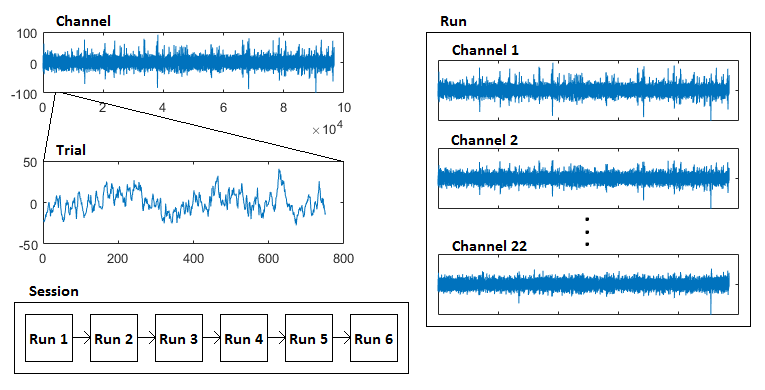
\includegraphics{figures/bciiv2a.png}
	\end{adjustbox}
	\caption{Sessions, runs, channels, trials, and the relations between them.}
	\label{fig:dataset}
\end{figure*}

We set up two pipelines to be compared. The first consists of artifact correction, followed by feature extraction with FBCSP and Random Forest classification. The second pipeline is identical but without the artifact correction step, i.e., just FBCSP and Random Forest. We run Random Forest with six predefined seeds and return the mean to ensure reproducibility.
To test the generality of the pipeline, we perform 6-fold cross-validation on the training data using five runs for training and one for validation. We run 200 iterations of Bayesian Optimization of select hyperparameters for each pipeline. The best hyperparameters from cross-validation for each pipeline is then used to construct the pipeline for the final evaluation, where we predict the labels for the test data. We repeat this for each subject. 
\cref{fig:results} shows the obtained accuracies with(C2) and without (C1) artifact correction for each subject.

\begin{table}[H]
	\begin{tabular}{@{}l|llll@{}} \toprule
		S					  & C1             & C2             & C3             & C4             \\ \midrule
		1                     & 83,04          & 82,29          & 81,42          & \textbf{83,85} \\
		2                     & 57,18          & 57,29          & 57,29          & \textbf{54,67} \\
		3                     & 78,18          & \textbf{79,16} & \textbf{79,16} & 75,64          \\
		4                     & 65,74          & 63,83          & 65,05          & \textbf{67,71} \\
		5                     & \textbf{58,85} & 55,21          & 55,21          & 56,94          \\
		6                     & \textbf{50,23} & 45,72          & 48,03          & 48,18          \\
		7                     & \textbf{68,75} & 68,69          & 68,69          & 67,94          \\
		8                     & 74,54          & 74,54          & \textbf{74,65} & 74,48          \\
		9                     & \textbf{75,64} & 72,97          & 72,80          & \textbf{75,64} \\ \bottomrule
	\end{tabular}
	\centering
	\caption{Accuracies for the best runs using 4 different setups. C1 is the baseline testing without OACL, C2 is 200 iterations of BO with OACL, C3 is 300 iterations of BO with OACL, C4 is 200 iterations with fixed parameters}
	\label{fig:results}
\end{table}

With 200 iterations the artifact correction did not overall yield better results than with no artifact correction and, in fact performed worse on some subjects. One possible cause may be that optimizing 27 parameters over 200 iterations is not a large enough budget to find optimal values for all hyperparameters, since the search space for 27 parameters is much larger than the search space for the 2 parameters optimized in the pipeline with no artifact correction. For this reason, we increased the iterations from 200 to 300 to see if this would yield improved results as illustrated in \cref{fig:i300}. As can be seen, the accuracy increased for three subjects, decreased for two, and remained the same for four. This indicates that 300 iterations are still not enough to optimize over such a large search space.


Because our objective is to determine whether removing the artifact signal from the raw signal yields improvements in classification accuracy, we manually set the non-artifact correction parameters to the best obtained values found in the non-correction evaluations, instead of further increasing the number of iterations. This introduces the assumption that good parameters without OACL are also good with OACL. Therefore, we now optimize the $\theta$ parameters to find the values that yield the highest accuracy. The results of running 200 iterations with this assumption are shown in \cref{fig:results}, as C4. \todo{discuss these results when we get them}

To determine the significance of these results we use the Wilcoxon signed-rank test. \Cref{fig:wilcoxon} shows the results of the test.



\subsection{Discussion}\label{sec:discussion}
% OACL ranges, may not only remove Ocular artifacts.
In the original OACL paper by \citep{li2015ocular}, the relative height ranges specified in \cref{eq:ranges} were determined by manual inspection of the characteristics of ocular artifacts. Since we generalized this as an optimization of hyperparameters, the found ranges are no longer guaranteed to be optimal in regards to ocular artifacts, but instead optimized for correcting the artifacts that most negatively affects the classification results. In fact, since we optimize the ranges for maximal classification accuracy, the method may be removing parts of the signal that are technically not artifacts, but removing them increases the performance of the classification model.

% Optimizing BO settings, and changing the kernel
Moreover, we have run Bayesian optimization with the default settings with regards to exploration vs. exploitation. Since running experiments on the pipeline with OACL is relatively expensive, it would be better to tune BO to spend more time on selecting the best candidate future sample to perform the next experiment on. The most used kernel for optimization problems used with BO is the squared exponential, this is however not always a good kernel, since sampling from a GP with this kernel, often will result in a unrealistic smooth function. Therefore we use Matérn 5/2 which is proposed in \citep{snoek2012practical}. Although this kernel function will be less smooth than the standard squared exponential, it might not be a suitable candidate for out optimization problem. In fact, BO might not even be possible with the domain of our parameters. BO assumes that input parameters with values close to each other, will have relatively similar outputs. Since our input space contains variables from many different algorithms, including FB, CSP and OACL, this assumption might however not hold. 

% Removing residual artifacts
As explained in \cite{hoffmann2008correction}, residual artifacts were still present after noise reduction methods were applied. We have also observed that residual artifacts are present, this can be seen in \cref{fig:oacl-signals}, where an event is registered around $x \approx 170$, but the following desynchronization/synchronization is not registered. A way that this could be handled is to always check if a residual artifact is present when an artifact is registered that, and mark it. These signals might need a separate $\theta$, since the signature of these artifacts is quite different from the artifacts introduced by eye blinks.

Since OACL is not restricted to finding ocular artifacts, a generalization of theta values for each channel, might not be optimal. This is due to the difference in how various artifacts shows in EEG data. A better way, might be to construct a classifier for artifacts, and use a different theta value for each such artifact. The classifier will then be used in the cleaning of new EEG signals, to remove just the right amount of artifact signal, based on the type of artifact. Furthermore, theta values are found based on optimization through BO. An alternative would be optimization through logistic regression. 
Since OACL is not restricted to finding ocular artifacts, a generalization of theta values for each channel, might not be optimal. This is due to the difference in how various artifacts shows in EEG data. A better way, might be to construct a classifier for artifacts, and use a different theta value for each such artifact. The classifier will then be used in the cleaning of new EEG signals, to remove just the right amount of artifact signal, based on the type of artifact. Furthermore, theta values are found based on optimization through BO.

An alternative would be optimization through logistic regression as proposed in the original OACL method by \citet{li2015ocular}. Even though their technique considered only binary classification, it would be possible to expand their logistic regression approach to the multi-class case, by applying an one-vs-rest algorithm to construct 4-binary classifiers. This should reduce the bayesian optimization search space, and increase the results of applying the ocular artifact correction.

% Using more oacl ranges
\todo{integrate the paragraphs below with discussion}
In this study we used just one range for OACL, but the method can easily be extended to use and optimize multiple ranges. That would likely increase the accuracy further, since different artifacts show up in different ranges. Each range adds to the dimensionality of the search space. Alternatively, a wavelet transform approach could be used for the removal step \citep{krishnaveni2006automatic}.

% More clever use of filter bank
The filter bank can be improved by optimizing over a wider variety of sub-bands, e.g., by mixing sub-bands with differing spans such as [4-8] and [8-11]. This would increase the complexity of the input space., which in turn would make the optimization of all parameters harder. 

%------------------------------------------------

\section{Conclusion}
The existence of artifacts is a persistent problem in EEG data that is detrimental to the efficacy of BCI systems. We considered the negative effect of ocular artifacts on motor imagery classification of 4-class EEG. As a possible solution to the problem, we presented a method for ocular artifact correction in multi class EEG data, as an extension to the binary class ocular artifact correction method OACL\citep{li2015ocular}. Furthermore, we showed that the hyperparameters that was manually determined in OACL, can be automatically tuned by application of Bayesian Optimization algorithm. By testing the ocular artifact correction on the BCI Competition dataset IV2a, we  we found that the best hyperparameters found after 200-300 iterations did not improve classification performance compared to classification without application of the ocular artifact correction method. We discuss that reasons for this include the problematically large optimization space over filtering parameters and that filtering parameters may not be generalizable over several trials.

Possible improvements for future work are adapting the logistic regression approach used by \citep{li2015ocular} for multi-class estimation of filtering parameters. Secondly, the detection and correction of the residual as a subprocess to the main artifact correction process. 
%Recapitulates the problem and the contribution.
%Assesses the significance of the contribution.
%Suggests and outlines future work, open problems, etc.

\section{Acknowledgement}
We thank Felipe Soares da Costa for valuable feedback. We would also like to thank Aalborg University for lending us hardware for testing program configurations.

%----------------------------------------------------------------------------------------
%	REFERENCE LIST
%----------------------------------------------------------------------------------------

\begin{thebibliography}{99} % Bibliography - this is intentionally simple in this template
 
@article{blankertz2008optimizing,
	title={Optimizing spatial filters for robust EEG single-trial analysis},
	author={Blankertz, Benjamin and Tomioka, Ryota and Lemm, Steven and Kawanabe, Motoaki and Muller, Klaus-Robert},
	journal={Signal Processing Magazine, IEEE},
	volume={25},
	number={1},
	pages={41--56},
	year={2008},
	publisher={IEEE}
}
\end{thebibliography}

%----------------------------------------------------------------------------------------

\end{multicols}

\end{document}
